\section{Introduction}

\subsection{The scalar meson $f_{0}(980)$ and $a_{0}(980)$}
\label{f0-a0-discussion}
\par{
    The Constituent Quark Model ahs been very successful in the past few decades by explaining how hadrons are made up.
    Base on this model, the nonets of pseudo-scalar, vector and tensor mesons are now well identified.
    However, the idenfitication of the scalar mesons is still uncertain due to the broad widths and the lack of a distincitive angular distribution.
    Among the candicates for the spin-parity $J^{PC}=0^{++}$ nonet, the parameters of some states such as $f_{0}(980)$ and $a_{0}(980)$ are not well measured.
    For $f_{0}(980)$, as it is very close to $K\bar{K}$ threshold and has strong coupling to $\pi\pi$ and $K\bar{K}$ final states, its parameters are still uncertain.
    
    
    According to the amplitude analysis of $D_{s}^{+} \rightarrow \pi^{+}\pi^{0}\eta$ ~\cite{Doc-DB-682-v7}, they observed the decay $D_{s}^{+} \rightarrow a_{0}(980)^{0}\pi^{+}$ and the contribution from $a_{0}(980)^{0}$ should also effect the $K^{+}K^{-}$ $\mathcal{S}$ wave shape in the $D_{s}^{+} \rightarrow K^{+}K^{-}\pi^{+}$ decay.
    So in this analysis, we have to take in account not only $f_{0}(980)$ but also $a_{0}(980)$ in the $K^{+}K^{-}$ $\mathcal{S}$ wave.  
    However, $f_{0}(980)$ and $a_{0}(980)$ are very close to each other and it is very difficutl to distinguith them without any extra input.
    
    
    From the Dalitz plot analysis of $D_{s}^{+} \rightarrow \pi^{+}\pi^{-}\pi^{+}$, we can get the branching fraction of $D_{s}^{+}$ decays to $f_{0}(980)\pi^{+}$ and then $f_{0}(980)$ decays to $\pi^{+}\pi^{-}$ is $\mathcal{B}(D_{s}^{+} \rightarrow f_{0}(980)\pi^{+}, f_{0}(980) \rightarrow \pi^{+}\pi^{-})$.
    Then if we know the the branching ratio of $\Gamma_{f_{0}(980)}(K^{+}K^{-})/\Gamma_{f_{0}(980)}(\pi^{+}\pi^{-})$, it is easy to obtain:
    \begin{equation}
        \begin{math}
            \mathcal{B}(D_{s}^{+} \rightarrow f_{0}(980)\pi^{+}, f_{0}(980) \rightarrow K^{+}K^{-}) =\mathcal{B}(D_{s}^{+} \rightarrow f_{0}(980)\pi^{+}, f_{0}(980) \rightarrow \pi^{+}\pi^{-})  \frac{\Gamma_{f_{0}(980)}(K^{+}K^{-})}{ \Gamma_{f_{0}(980)}(\pi^{+}\pi^{-})}. \label{bf-f0}
        \end{math}
    \end{equation}
    
    In a similar way, we can obtain:
    \begin{equation}
        \begin{math}
            \mathcal{B}(D_{s}^{+} \rightarrow a_{0}(980)\pi^{+}, a_{0}(980) \rightarrow K^{+}K^{-}) =\mathcal{B}(D_{s}^{+} \rightarrow a_{0}(980)\pi^{+}, a_{0}(980) \rightarrow \pi^{0}\eta)  \frac{\Gamma_{a_{0}(980)}(K^{+}K^{-})}{ \Gamma_{a_{0}(980)}(\pi^{0}\eta)}. \label{bf-a0} 
        \end{math}
    \end{equation}
    
    Then, obviously, the ratio of fit fractions of $D_{s}^{+} \rightarrow f_{0}(980)\pi^{+}$ and $D_{s}^{+} \rightarrow a_{0}(980)\pi^{+}$ $\Gamma$ is: 
    \begin{equation}
        \begin{math}
            \Gamma  =\frac{\mathcal{B}(D_{s}^{+} \rightarrow f_{0}(980)\pi^{+}, f_{0}(980) \rightarrow \pi^{+}\pi^{-})  \frac{\Gamma_{f_{0}(980)}(K^{+}K^{-})}{ \Gamma_{f_{0}(980)}(\pi^{+}\pi^{-})}}{\mathcal{B}(D_{s}^{+} \rightarrow a_{0}(980)\pi^{+}, a_{0}(980) \rightarrow \pi^{0}\eta)  \frac{\Gamma_{a_{0}(980)}(K^{+}K^{-})}{ \Gamma_{a_{0}(980)}(\pi^{0}\eta)}}. \label{a0-f0-bf}
        \end{math}
    \end{equation}
    
    If we can get the value of $\Gamma$ in Eq. \ref{a0-f0-bf}, it's possible to fix the ratio in amplitude analysis and then distinguith $f_{0}(980)$ and $a_{0}(980)$ at the low end of $K^{+}K^{-}$ mass spectrum.
    Using isopin relations,  the relation between $\Gamma_{f_{0}(980)}(\pi\pi) /  \Gamma_{f_{0}(980)}(\pi\pi+K\bar{K})$ and $\Gamma_{f_{0}(980)}(K^{+}K^{-}) / \Gamma_{f_{0}(980)}(\pi^{+}\pi^{-})$ is:
    \begin{equation}
        \frac{\Gamma_{f_{0}(980)}(K^{+}K^{-})}{ \Gamma_{f_{0}(980)}(\pi^{+}\pi^{-})} =  \frac{3}{4} \cdot \left[\frac{1}{\frac{\Gamma_{f_{0}(980)}(\pi\pi)} {\Gamma_{f_{0}(980)}(\pi\pi)+\Gamma_{f_{0}(980)}(K\bar{K})}} -1\right]. \label{f0-KK-pipi-relation}
    \end{equation}
    However the value of $\Gamma_{f_{0}(980)}(K^{+}K^{-}) / \Gamma_{f_{0}(980)}(\pi^{+}\pi^{-})$ is not well measured as is shown in following Table \ref{f0-KK-pipi} from Ref. ~\cite{PDG2018}.
    So we have to extract the $\mathcal{S}$ wave line shape at the low end of $K^{+}K^{-}$ mass spectrum in a quasi-model-independent way.
    In other words, we take $a_{0}(980)$ and $f_{0}(980)$ as a whole.

\begin{table}
    \caption{The $f_{0}(980)$ branching ratio $\Gamma_{f_{0}(980)}(\pi\pi) / \left[ \Gamma_{f_{0}(980)}(\pi\pi)+\Gamma_{f_{0}(980)}(K\bar{K})\right]$}
    \label{f0-KK-pipi}
    \begin{center}
        \begin{tabular}{cccc}
            \toprule
            VALUE &         TECN & COMMENT\\
            \hline
            $0.52\pm0.12$ &             BABR    & $B^{\pm} \rightarrow K^{\pm}\pi^{\pm}\pi^{\mp}$   ~\cite{pipi-KK-1} \\
            $0.75_{-0.13}^{+0.11}$ &    BES2    & $\chi_{c0} \rightarrow 2\pi^{+}2\pi^{-}, \pi^{+}\pi^{-}K^{+}K^{-}$   ~\cite{pipi-KK-2} \\
            $0.84\pm0.02$ &             SPEC    & Combined fit   ~\cite{pipi-KK-3} \\
            \bottomrule
        \end{tabular}
    \end{center}
\end{table}





}

\subsection{The $D_{s}^{+} \rightarrow K^{+}K^{-}\pi^{+}$ decay}
\par{

    The decay $D_{s}^{+} \rightarrow K^{+}K^{-}\pi^{+}$ is a Cabibbo-favored (CF) channel and has a large branching fraction for the $D_{s}$ meson.
    Thus, this decay channel is usually used to normalize measurements of decay chains involving charm quarks.
    Fig. \ref{Feynman-dia} illustrates main Feynman diagrams related to the decay.
    \begin{figure*}[h]
        \centering
        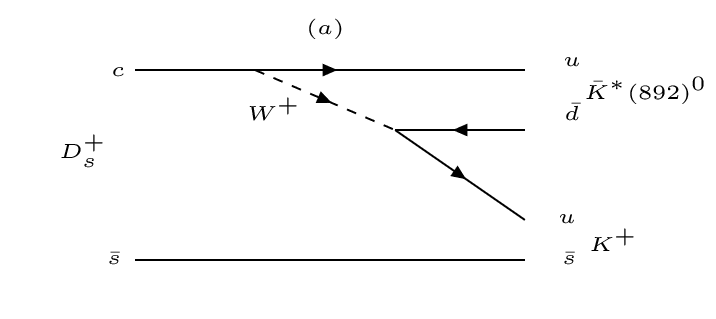
\includegraphics[width=0.45\textwidth]{plot/Fa.PNG}
        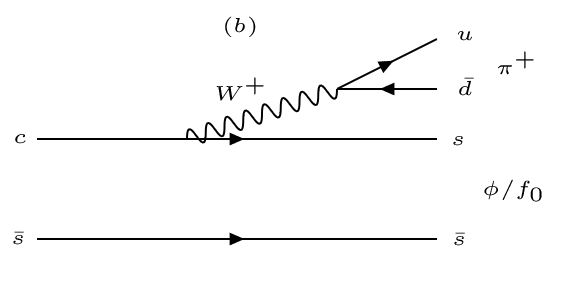
\includegraphics[width=0.45\textwidth]{plot/Fb.PNG}
        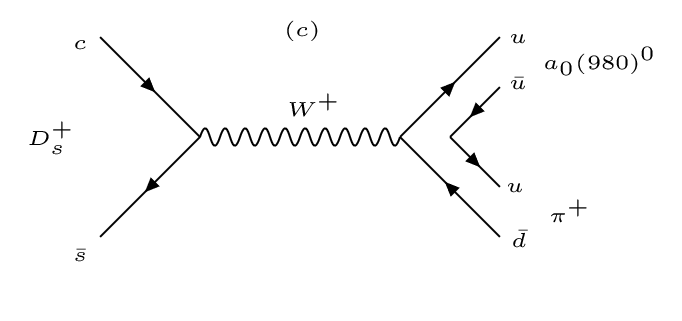
\includegraphics[width=0.45\textwidth]{plot/Fc.PNG}
        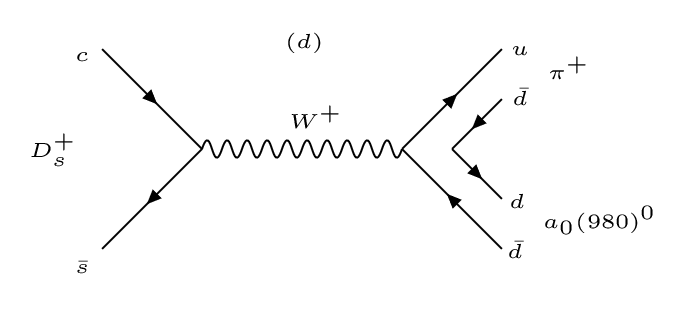
\includegraphics[width=0.45\textwidth]{plot/Fd.PNG}
        %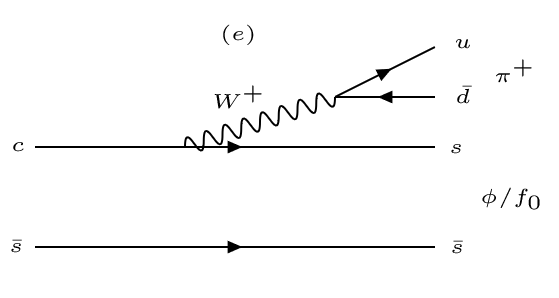
\includegraphics[width=0.45\textwidth]{plot/Fe.PNG}
        \caption{Main Feynman tree diagrams associated with $D_{s}^{+} \rightarrow K^{+}K^{-}\pi^{+}$ decay.}
        \label{Feynman-dia}
    \end{figure*}
    The main contribution comes from the tree diagram with an internal $W^{+}$ emission(Fig. \ref{Feynman-dia}(a)), that describes the $D_{s}^{+} \rightarrow \bar{K}^{*}(892)^{0}K^{+}$ decay, 
    and the diagram with an external $W^{+}$ emission(Fig. \ref{Feynman-dia}(b)), that describes the diagram $D_{s}^{+} \rightarrow \phi\pi^{+}/ f_{0}\pi^{+}$, 
    and the diagram with W-annihilation(Fig. \ref{Feynman-dia}(c) and Fig. \ref{Feynman-dia}(d)), that describes the decay $D_{s} \rightarrow a_{0}(980)^{0}\pi^{+}$.
}
    
\subsection{Amplitude analysis}
\par{
    Knowledge of the decay amplitude allows us to properly account for interference effects when measuring absolute hadronic branching fractions of $D_{s}$ mesons.
    Amplitude analysis of this decay can help us to understand the interference effects and so an amplitude analysis is necessary.
Below is the table of previous analyses of this decay channel.}

\begin{table}
    \caption{previous analyses of this decay channel.}
    \label{PreviousAnalyses}
    \begin{center}
        \begin{tabular}{cccc}
            \toprule\toprule
            Decay mode & Fit fraction(BABAR)  & Fit fraction(CLEO-c)  & Fit fraction(E687)\\
            \midrule
            $D_{s}^{+} \rightarrow \bar{K}^{*}(892)^{0}K^{+}$              & 47.9$\pm$0.5$\pm$0.5  & 47.4$\pm$1.5$\pm$0.4& 47.8$\pm$4.6$\pm$4.0 \\
            $D_{s}^{+} \rightarrow \phi(1020)\pi^{+}$                      & 41.4$\pm$0.8$\pm$0.5  & 42.2$\pm$1.6$\pm$0.3& 39.6$\pm$3.3$\pm$4.7 \\
            $D_{s}^{+} \rightarrow f_{0}(980)\pi^{+}/a_{0}(980)\pi^{+}$    & 16.4$\pm$0.7$\pm$2.0  & 28.2$\pm$1.9$\pm$1.8& 11.0$\pm$3.5$\pm$2.6 \\
            $D_{s}^{+} \rightarrow \bar{K}^{*}_{0}(1430)^{0}K^{+}$         & 2.4$\pm$0.3$\pm$1.0   & 3.9$\pm$0.5$\pm$0.5 & 9.3$\pm$3.2$\pm$3.2  \\
            $D_{s}^{+} \rightarrow f_{0}(1710)\pi^{+}$                     & 1.1$\pm$0.1$\pm$0.1   & 3.4$\pm$0.5$\pm$0.3 & 3.4$\pm$2.3$\pm$3.5  \\
            $D_{s}^{+} \rightarrow f_{0}(1370)\pi^{+}$                     & 1.1$\pm$0.1$\pm$0.2   & 4.3$\pm$0.6$\pm$0.5 & ...                  \\ 
            $\begin{matrix}\sum FF(\%)\end{matrix}$                          & 110.2$\pm$0.6$\pm$2.0 & 129.5$\pm$4.4$\pm$2.0 & 111.1\\
                \midrule
                $\chi^{2}/NDF$                                                  & $\frac{2843}{2305-14}=1.2$ & $\frac{178}{117}=1.5$ & $\frac{50.2}{33}=1.5$\\
                \midrule
                Events                                                         &$96307\pm369$          &$12226\pm22$  &$701\pm36$\\
                \bottomrule\bottomrule
            \end{tabular}
        \end{center}
    \end{table}


    From Table\ref{PreviousAnalyses}~\cite{2011BARBAR}, we can see an obvious difference of decay fraction of $f_{0}(980)\pi^{+}$ between BARBAR and CLEO-c. E687 used about 700 events and the E687 model did not take $f_{0}(1370)\pi^{+}$ into account. For CLEO-c, about 14400 events with purity about 84.9\% were selected with single tag method. The analysis of BARBAR used about 100000 events with purity about 95\%. In this analysis with double tag method, we can get a nearly background free data sample, that will be good to perform the amplitude analysis.
}

    \iffalse
    As shown in Fig. \ref{fig:lambc_cs} and Figure~\ref{fig:lambc_cs_bes3}, at the energy of 4.6\,GeV, cross section of producing $\lambdacp\lambdacm$ pair in $\ee$ collisions is $\sigma(\ee\to\lambdacp\lambdacm)=0.38\pm0.13\,\rm{nb}$ measured by BELLE~\cite{Pakhlova:2008vn} and $\sigma(\ee\to\lambdacp\lambdacm)=0.253\pm0.023\,\rm{nb}$ measured by BESIII~\cite{Weiping:lineshape}.\\

    %%%%%%%%%%%%%%%%%%%%%%%%%%%%


    %%%%%%%%%%%%%%%%%%%%%%%%%%%%
    \begin{figure*}[h]
        \centering
        \includegraphics[width=0.45\textwidth]{bes3_lineshape.eps}
        \caption{Cross sections of $\ee\to\lambdacp\lambdacm$ measured by BESIII.}
        \label{fig:lambc_cs_bes3}
    \end{figure*}
    %%%%%%%%%%%%%%%%%%%%%%%%%%%%%
    \fi
